%%%%%%%%%%%%%%%%%%%%%%%%%%%%%%%%%%%%%%%%%%%%%%%%%%%%%%%%%%%%%%%%%%%%%%%%%%%%%%%%
%% Plantilla de memoria en LaTeX para la ETSIT - Universidad Rey Juan Carlos
%%
%% Por Gregorio Robles <grex arroba gsyc.urjc.es>
%%     Grupo de Sistemas y Comunicaciones
%%     Escuela Técnica Superior de Ingenieros de Telecomunicación
%%     Universidad Rey Juan Carlos
%% (muchas ideas tomadas de Internet, colegas del GSyC, antiguos alumnos...
%%  etc. Muchas gracias a todos)
%%
%% La última versión de esta plantilla está siempre disponible en:
%%     https://github.com/gregoriorobles/plantilla-memoria
%%
%% Para obtener PDF, ejecuta en la shell:
%%   make
%% (las imágenes deben ir en PNG o JPG)

%%%%%%%%%%%%%%%%%%%%%%%%%%%%%%%%%%%%%%%%%%%%%%%%%%%%%%%%%%%%%%%%%%%%%%%%%%%%%%%%

\documentclass[a4paper, 12pt]{book}
%\usepackage[T1]{fontenc}

\usepackage[a4paper, left=2.5cm, right=2.5cm, top=3cm, bottom=3cm]{geometry}
\usepackage{times}
\usepackage[utf8]{inputenc}
\usepackage[spanish]{babel} % Comenta esta línea si tu memoria es en inglés
\usepackage{url}
%\usepackage[dvipdfm]{graphicx}
\usepackage{graphicx}
\usepackage{float}  %% H para posicionar figuras
\usepackage[nottoc, notlot, notlof, notindex]{tocbibind} %% Opciones de índice
\usepackage{latexsym}  %% Logo LaTeX
\usepackage{listings} %% Para que el codigo quede bonito

\title{Memoria del Proyecto}
\author{Nombre del autor}

\renewcommand{\baselinestretch}{1.5}  %% Interlineado

\begin{document}

\renewcommand{\refname}{Bibliografía}  %% Renombrando
\renewcommand{\appendixname}{Apéndice}

%%%%%%%%%%%%%%%%%%%%%%%%%%%%%%%%%%%%%%%%%%%%%%%%%%%%%%%%%%%%%%%%%%%%%%%%%%%%%%%%
% PORTADA

\begin{titlepage}
\begin{center}
\includegraphics[scale=0.8]{img/URJ_logo_Color_POS.png}

\vspace{1.75cm}

\Large
GRADO EN INGENIERÍA EN SISTEMAS AUDIOVISUALES Y MULTIMEDIA

\vspace{0.4cm}

\large
Curso Académico 2020/2021

\vspace{0.8cm}

Trabajo Fin de Grado

\vspace{2.5cm}

\LARGE
TÍTULO DEL TRABAJO EN MAYÚSCULAS

\vspace{4cm}

\large
Autor : Jorge De Pablo Martínez \\
Tutor : Dr. Gregorio Robles Martínez
\end{center}
\end{titlepage}

\newpage
\mbox{}
\thispagestyle{empty} % para que no se numere esta pagina


%%%%%%%%%%%%%%%%%%%%%%%%%%%%%%%%%%%%%%%%%%%%%%%%%%%%%%%%%%%%%%%%%%%%%%%%%%%%%%%%
%%%% Para firmar
\clearpage
\pagenumbering{gobble}
\chapter*{}

\vspace{-4cm}
\begin{center}
\LARGE
\textbf{Trabajo Fin de Grado}

\vspace{1cm}
\large
Título del Trabajo con Letras Capitales para Sustantivos y Adjetivos

\vspace{1cm}
\large
\textbf{Autor :} Jorge De Pablo Martínez \\
\textbf{Tutor :} Dr. Gregorio Robles Martínez

\end{center}

\vspace{1cm}
La defensa del presente Proyecto Fin de Carrera se realizó el día \qquad$\;\,$ de \qquad\qquad\qquad\qquad \newline de 202X, siendo calificada por el siguiente tribunal:


\vspace{0.5cm}
\textbf{Presidente:}

\vspace{1.2cm}
\textbf{Secretario:}

\vspace{1.2cm}
\textbf{Vocal:}


\vspace{1.2cm}
y habiendo obtenido la siguiente calificación:

\vspace{1cm}
\textbf{Calificación:}


\vspace{1cm}
\begin{flushright}
Fuenlabrada, a \qquad$\;\,$ de \qquad\qquad\qquad\qquad de 202X
\end{flushright}

%%%%%%%%%%%%%%%%%%%%%%%%%%%%%%%%%%%%%%%%%%%%%%%%%%%%%%%%%%%%%%%%%%%%%%%%%%%%%%%%
%%%% Dedicatoria

\chapter*{}
\pagenumbering{Roman} % para comenzar la numeracion de paginas en numeros romanos
\begin{flushright}
\textit{Dedicado a \\
mi familia / mi abuelo / mi abuela}
\end{flushright}

%%%%%%%%%%%%%%%%%%%%%%%%%%%%%%%%%%%%%%%%%%%%%%%%%%%%%%%%%%%%%%%%%%%%%%%%%%%%%%%%
%%%% Agradecimientos

\chapter*{Agradecimientos}
%\addcontentsline{toc}{chapter}{Agradecimientos} % si queremos que aparezca en el índice
\markboth{AGRADECIMIENTOS}{AGRADECIMIENTOS} % encabezado 

Aquí vienen los agradecimientos\ldots Aunque está bien acordarse de la pareja, no hay que olvidarse de dar las gracias a tu madre, que aunque a veces no lo parezca disfrutará tanto de tus logros como tú\ldots 
Además, la pareja quizás no sea para siempre, pero tu madre sí.

%%%%%%%%%%%%%%%%%%%%%%%%%%%%%%%%%%%%%%%%%%%%%%%%%%%%%%%%%%%%%%%%%%%%%%%%%%%%%%%%
%%%% Resumen

\chapter*{Resumen}
%\addcontentsline{toc}{chapter}{Resumen} % si queremos que aparezca en el índice
\markboth{RESUMEN}{RESUMEN} % encabezado

El lenguaje unificado modelado es en la actualidad la herramienta más utilizada en el modelado de software. No obstante, los diagramas y aspectos conceptuales del mismo pueden utilizarse para otros entornos, como el educativo.  

La aplicación web Ghymkhana App 

\begin{itemize}
  \item ¿De qué va este proyecto? ¿Cuál es su objetivo principal?
  \item ¿Cómo se ha realizado? ¿Qué tecnologías están involucradas?
  \item ¿En qué contexto se ha realizado el proyecto? ¿Es un proyecto dentro de un marco general?
\end{itemize}

Lo mejor es escribir el resumen al final.

%%%%%%%%%%%%%%%%%%%%%%%%%%%%%%%%%%%%%%%%%%%%%%%%%%%%%%%%%%%%%%%%%%%%%%%%%%%%%%%%
%%%% Resumen en inglés

\chapter*{Summary}
%\addcontentsline{toc}{chapter}{Summary} % si queremos que aparezca en el índice
\markboth{SUMMARY}{SUMMARY} % encabezado

Here comes a translation of the ``Resumen'' into English. 
Please, double check it for correct grammar and spelling.
As it is the translation of the ``Resumen'', which is supposed to be written at the end, this as well should be filled out just before submitting.


%%%%%%%%%%%%%%%%%%%%%%%%%%%%%%%%%%%%%%%%%%%%%%%%%%%%%%%%%%%%%%%%%%%%%%%%%%%%%%%%
%%%%%%%%%%%%%%%%%%%%%%%%%%%%%%%%%%%%%%%%%%%%%%%%%%%%%%%%%%%%%%%%%%%%%%%%%%%%%%%%
% ÍNDICES %
%%%%%%%%%%%%%%%%%%%%%%%%%%%%%%%%%%%%%%%%%%%%%%%%%%%%%%%%%%%%%%%%%%%%%%%%%%%%%%%%

% Las buenas noticias es que los índices se generan automáticamente.
% Lo único que tienes que hacer es elegir cuáles quieren que se generen,
% y comentar/descomentar esa instrucción de LaTeX.

%%%% Índice de contenidos
\tableofcontents 
%%%% Índice de figuras
\cleardoublepage
%\addcontentsline{toc}{chapter}{Lista de figuras} % para que aparezca en el indice de contenidos
\listoffigures % indice de figuras
%%%% Índice de tablas
%\cleardoublepage
%\addcontentsline{toc}{chapter}{Lista de tablas} % para que aparezca en el indice de contenidos
%\listoftables % indice de tablas


%%%%%%%%%%%%%%%%%%%%%%%%%%%%%%%%%%%%%%%%%%%%%%%%%%%%%%%%%%%%%%%%%%%%%%%%%%%%%%%%
%%%%%%%%%%%%%%%%%%%%%%%%%%%%%%%%%%%%%%%%%%%%%%%%%%%%%%%%%%%%%%%%%%%%%%%%%%%%%%%%
% INTRODUCCIÓN %
%%%%%%%%%%%%%%%%%%%%%%%%%%%%%%%%%%%%%%%%%%%%%%%%%%%%%%%%%%%%%%%%%%%%%%%%%%%%%%%%

\cleardoublepage
\chapter{Introducción}
\label{sec:intro} % etiqueta para poder referenciar luego en el texto con ~\ref{sec:intro}
\pagenumbering{arabic} % para empezar la numeración de página con números

La siguiente memoria recoge el trabajo realizado durante el desarrollo de Gymkhana App. Se trata de una aplicación web diseñada y orientada para que niños y niñas puedan disfrutar de sencillos juegos a la vez que aprender conceptos de lenguaje unificado modelado.

\section{Contexto}
\label{sec:seccion}
Gymkhana App es una aplicación web con simples juegos que consisten en la resolución de diagramas UML (lenguaje unificado modelado, de las siglas en inglés \emph{Unified Modeling Language}), o extracción de las respuestas a través del análisis de estos. 

La idea surge bajo la premisa de fomentar y ayudar en el desarrollo de habilidades como el seguimiento de flujo, pensamiento lógico, simplificación y análisis de situaciones complejas y la resolución de problemas mediante la división de estos en un conjunto de actividades estructurales que juntas forman una solución. 

Los mini-juegos consisten en resolución de sencillos enigmas que se resuelven combinando sus habilidades con diagramas UML. El nivel elegido en esta primera versión está orientado para niños de entre nueve y doce años. 

Se trata de divulgar y enseñar conceptos de UML y que, a al vez, los más jóvenes se familiaricen con estos últimos a través los sencillos juegos y retos que contiene Gymkhana App. 


\section{Estructura de la memoria}
\label{sec:estructura}

La memoria de este trabajo esta estructurada de la siguiente manera: 

\begin{itemize}
  \item Capítulo 1. Introducción. En el primer capítulo se hace una introducción al proyecto y se exponen las ideas básicas del mismo además de definir su estructura. 
  
  \item En el capítulo~\ref{chap:objetivos} (ojo, otra referencia automática) se muestran los objetivos del proyecto.
  
  \item A continuación se presenta el estado del arte en el capítulo~\ref{chap:estado}.
  
  \item \ldots
\end{itemize}



%%%%%%%%%%%%%%%%%%%%%%%%%%%%%%%%%%%%%%%%%%%%%%%%%%%%%%%%%%%%%%%%%%%%%%%%%%%%%%%%
%%%%%%%%%%%%%%%%%%%%%%%%%%%%%%%%%%%%%%%%%%%%%%%%%%%%%%%%%%%%%%%%%%%%%%%%%%%%%%%%
% OBJETIVOS %
%%%%%%%%%%%%%%%%%%%%%%%%%%%%%%%%%%%%%%%%%%%%%%%%%%%%%%%%%%%%%%%%%%%%%%%%%%%%%%%%

\cleardoublepage % empezamos en página impar
\chapter{Objetivos} % título del capítulo (se muestra)
\label{chap:objetivos} % identificador del capítulo (no se muestra, es para poder referenciarlo)


\section{Objetivo general} % título de sección (se muestra)
\label{sec:objetivo-general} % identificador de sección (no se muestra, es para poder referenciarla)

El objetivo de este trabajo es desarrollar una aplicación web sencilla, limpia y clara enfocada para su uso por niños que aprendan y se familiaricen con el lenguaje unificado modelado y sus tipos de diagramas. El desarrollo del este proyecto se ha hecho con Django y apoyándose principalmente en otras tecnologías y servicios como Heroku, Git y Bootstrap.

\section{Objetivos específicos}
\label{sec:objetivos-especificos}

Los objetivos específicos se pueden entender como las tareas en las que se ha desglosado el objetivo general.
Y, sí, también vienen en.


\section{Planificación temporal}
\label{sec:planificacion-temporal}

A mí me gusta que aquí pongáis una descripción de lo que os ha llevado realizar el trabajo.
Hay gente que añade un diagrama de GANTT.
Lo importante es que quede claro cuánto tiempo llevas (tiempo natural, p.ej., 6 meses) y a qué nivel de esfuerzo (p.ej., principalmente los fines de semana).


%%%%%%%%%%%%%%%%%%%%%%%%%%%%%%%%%%%%%%%%%%%%%%%%%%%%%%%%%%%%%%%%%%%%%%%%%%%%%%%%
%%%%%%%%%%%%%%%%%%%%%%%%%%%%%%%%%%%%%%%%%%%%%%%%%%%%%%%%%%%%%%%%%%%%%%%%%%%%%%%%
% ESTADO DEL ARTE %
%%%%%%%%%%%%%%%%%%%%%%%%%%%%%%%%%%%%%%%%%%%%%%%%%%%%%%%%%%%%%%%%%%%%%%%%%%%%%%%%

\cleardoublepage
\chapter{Estado del arte}
\label{chap:estado}


La aplicación web en la que se basa este proyecto se ha desarrollado con diferentes tecnologías gratuitas y de código abierto (\emph{Open Source}), pero la piedra angular sobre la que se apoya todo el proyecto es sobre el lenguaje unificado modelado. 


\section{UML: Unified Modeling Language} 
\label{sec:seccion1}

El lenguaje unificado modelado, también conocido por sus siglas en inglés UML, es el lenguaje de modelado de software más utilizado actualmente. 

El modelado de software es una parte esencial en todo el proceso de desarrollo del software. Al igual que en el plano análogo de la construcción de rascacielos, los planos, mapas del sitio y modelos físicos cumplen un papel esencial en la finalización con éxito del proyecto, en el desarrollo de software el lenguaje unificado modelado es necesario para asegurarse de que la funcionalidad del producto final es completa y correcta, de que satisface las necesidades del usuario final y que el diseño del programa admite los requisitos de escalabilidad, solidez, seguridad, expansibilidad y otras importantes características de un software. 

Se puede definir como un lenguaje gráfico que tiene como finalidad documentar, construir, especificar y en definitiva visualizar un sistema. Así mismo, también ofrece un estándar con el que definir un sistema o modelo. 

Es importante destacar que UML no es un lenguaje de programación ni es programación estructurada, pues UML es un lenguaje de modelado con el que se definen métodos y procesos, es decir el lenguaje que describe el modelo.

Desde fue presentado el primer estándar UML en 1997 (UML 1.1) hasta día de hoy ha evolucionado, en el momento de redactar esta memoria la OMT\footnote{Object Management Group \url{https://www.omg.org/}}, organización que respalda UML, tiene formalmente liberada la versión 2.5.1, que es sobre la cual este proyecto se ha desarrollado.
Naturalmente entre medias de han aparecido y varias versiones menores las cual han ido actualizando y corrigiendo hasta la versión que se utiliza actualmente. Desde el año 2004, UML es un estándar aprobado por la ISO (ISO/IEC 19501:2005 Information technology — Open Distributed Processing — Unified Modeling Language) y en el año 2012 se actualizó la norma dando lugar a la ISO/IEC 19505-1, la última versión disponible en este momento.

En UML se definen distintos tipos de diagramas, los cuales muestran diferentes aspectos del modelo representado. 
Los dos tipos principales de diagramas son: diagramas \emph{estructurales} y diagramas de \emph{comportamiento}. En la Figura 3.1 se puede ve un "metadiagrama" donde están ordenados jerárquicamente los diferentes tipos de diagrama. 

\begin{figure}
	\centering
	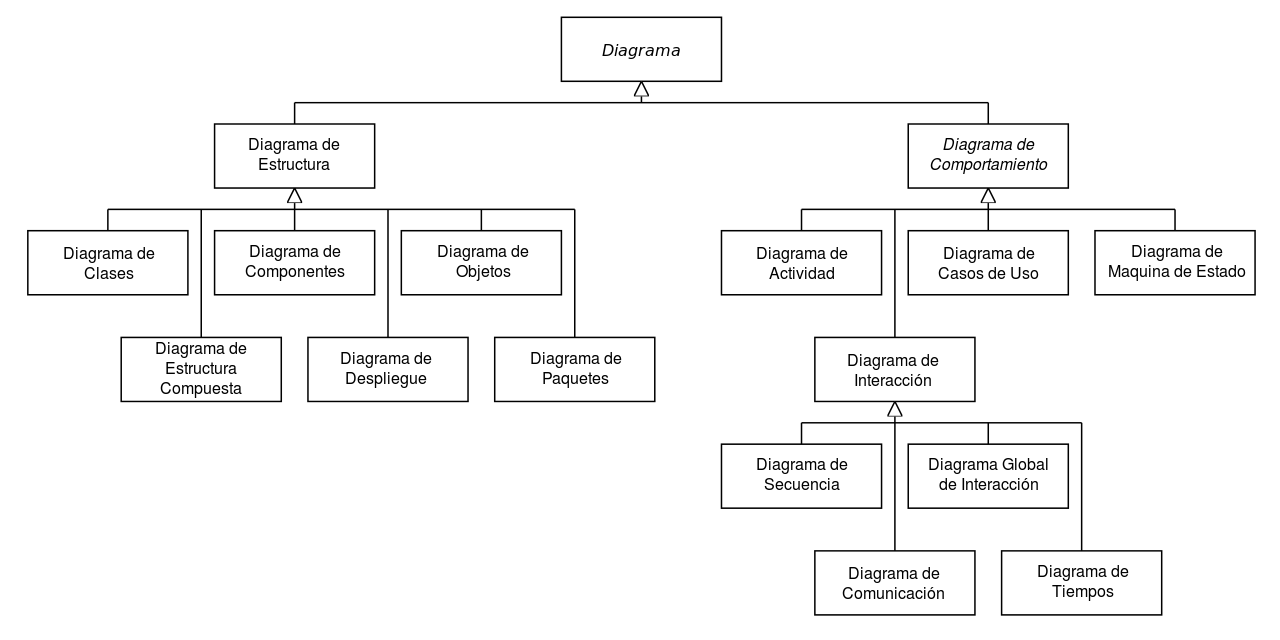
\includegraphics[width=16cm, keepaspectratio]{img/Uml_diagram.png}
	\caption{Jerarquía de diagramas en UML 2.2 (como diagrama de clases).}\label{fig:Uml_diagram}
\end{figure}

\subsection{Diagramas Estructurales}
Los diagramas estructurales muestran la estructura estática de los objetos en un sistema, es decir representan los elementos independientes del tiempo en un sistema. Los diagramas estructurales no muestran los detalles del comportamiento dinámico de un sistema, para ello existen los diagramas de comportamiento, sin embargo sí que pueden mostrar las relaciones entre los comportamientos definidos en la estructura.  

A continuación se describe brevemente cada uno de los diagramas pertenecientes a la familia de los diagramas estructurales que se muestran en la Figura 3.1: 

\subparagraph{Diagrama de clases}
Este tipo de diagramas proporciona los mecanismos para definir la estructura de un sistema estático. Muestra las clases del sistema, sus atributos, métodos y las relaciones y entre los objetos. 
\subparagraph{Diagrama de despliegue}
Esta clase de diagrama muestra la arquitectura de ejecución de un sistema. Incluyendo entornos de ejecución de hardware o software y el middleware que los conecta. Principalmente ayudan a entender y modelar la topología hardware de un sistema y como se despliega. 
\subparagraph{Diagrama de componentes} Los diagramas de componentes representan un sistema software dividido en componentes y muestra las dependencias entre los componentes. Son realmente útiles para ver qué componentes pueden compartirse entre sistemas o entre diferentes partes de un sistema.  
\subparagraph{Diagrama de objetos}
Este tipo de diagramas ofrece una vista parcial o completa de los objetos de un sistema. Es un gráfico de instancias que incluye objetos y datos. Estos diagramas están ligados a a los diagramas de clases, muestra el estado del sistema en un punto determinado del tiempo. 
\subparagraph{Diagrama de paquetes}
Representa las dependencias entre los paquetes que componen un sistema. Muestra como este está dividido en agrupaciones lógicas y las dependencias entre esas agrupaciones. Estos diagramas muestran la descomposición de la jerarquía lógica de un sistema.  
\subparagraph{Diagrama de estructura compuesta}
Esta clase de diagrama muestra la estructura interna de una clase y las relaciones e interacciones entre las distintas partes de la misma. Muestran el rol definido que tiene cada elemento y la estructura compuesta como el conjunto de esos elementos interconectados.

\subsection{Diagramas de Comportamiento}
Los diagramas de comportamiento muestran el comportamiento dinámico de un sistema, se puede describir como la serie de cambios que pueden existir en un sistema en un tiempo extraordinario.  
\subparagraph{Diagrama de actividad}
También conocidos como diagrama de flujo es la representación gráfica de un algoritmo o proceso. Representan flujos de trabajo paso a paso utilizando símbolos para representar cada uno de estos y flechas que conectan los símbolos para marcar el flujo de ejecución. 
\subparagraph{Diagrama de casos de uso}
Los diagramas de casos de usos describen los diferentes tipos de interacción que tiene alguien o algo con un determinado sistema, especificando el tipo de comunicación y comportamiento del mismo mediante la interacción con los usuarios y/u otros sistemas.
\subparagraph{Diagrama de interacción}
Este tipo de diagrama describen en detalle un determinado escenario de casos de uso. Ilustran la interacción entre el conjunto de objetos que cooperan en la realización de un proceso. 

\subparagraph{Diagrama de máquina de estados}
Un diagrama de máquina de estados, conocidos en ocasiones como diagrama de estados modela el comportamiento de un objeto. Especifican la secuencia de eventos que sufre este determinado objeto durante su tiempo de ejecución. 

%SE PODRIA AÑADIR EN LOS ANEXOS EJEMPLOS DE CADA UNO DE ELLOS ANEXO 2 


\section{Python}
Python es un lenguaje de programación interpretado, dinámico y multiplataforma con licencia de código abierto\footnote{Python Software Foundation License: \url{https://docs.python.org/3/license.html}}. Su máxima es hacer un lenguaje que sea fácilmente legible y con una empinada curva de aprendizaje. Python fue creado a principios de los 90s por Guido van Rossum en los Países Bajos, como curiosidad, saber que le debe su nombre gracias la afición que tenía su creador por el grupo de humoristas británicos Monty Python. 

\begin{figure}
	\centering
	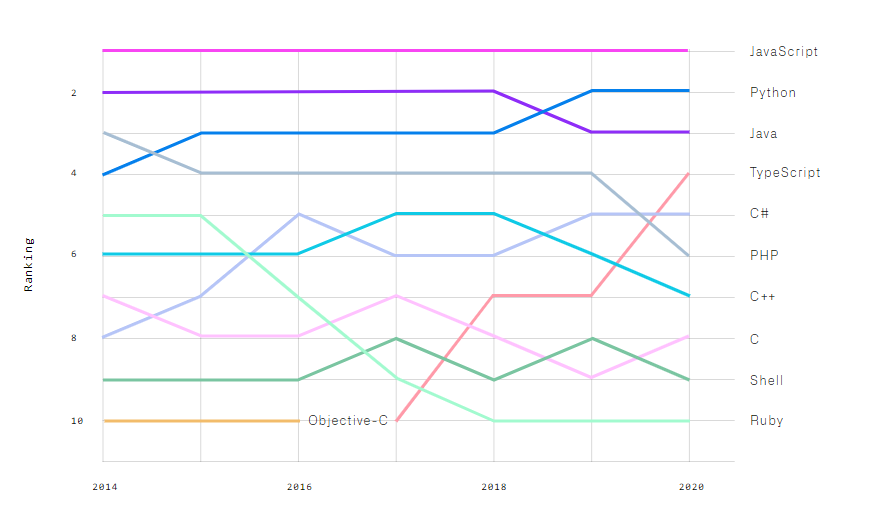
\includegraphics[width=18cm]{img/top_programing_languajes.png}
	\caption{Top uso de lenguajes de progrmación alojados en GitHub}
	\label{fig:Top_programming}
\end{figure}
%% (source:https://octoverse.github.com/#overview )

Dentro de sus características nos encontramos con que Python es: 
\begin{itemize}
	\item Interpretado: No es necesario que sea procesado por el compilador, se detectan errores en tiempo de ejecución 
	\item Multiparadigma: Soporta tanto programación funcional, como programación orientada objetos y también programación imperativa.  
	\item Tipado dinámico: Las variables se comprueban en tiempo de ejecución. 
	\item Flexible: No es obligatorio definir ni asignar variables antes de usarlas, es posible omitir parámetros, y sú única manera de definir la estructura del código en mediante indentación.
	\item Multiplataforma: Puede ejecutarse tanto en Linux, como Windows como macOS. 
\end{itemize}


Gracias a la versatilidad y fácil acceso a este lenguaje ha provocado que en los últimos años se haya vuelto muy relevante haciendo que sea uno de los principales y más importantes lenguajes de programación usados hoy en día. Como se puede ver en la Figura 3.2.
Actualmente su última versión estable es Python 3.9, pero este proyecto ha sido desarrollado usando la versión 3.7.3, ya que es una de las más populares y con más usuarios en activo. También cuenta con una versión anterior muy popular, Python 2, que es fue considerada \emph{"deprecated"} el 1 de enero de 2020. 

  
\section{Django}
Django es un framework de desarrollo web gratuito, de código abierto y escrito en Python. Fue lanzado en Julio de 2005 y comparte objetivos generales con Python buscando fundamentalmente poder desarrollar sitios web complejos de manera sencilla y accesible para el mayor número de personan posibles. Django funciona bajo Python, es decir, que para poder trabajar con Django es necesario tener instalado Python. 

Un framework, traduciéndolo al castellano, viene a ser un marco de trabajo, una especie de ecosistema formado por un  conjunto de herramientas, librerías y buenas prácticas para crear aplicaciones, en este caso para desarrollar aplicaciones web. 

El framework de Django en concreto nos permite crear sitios web con un cierto grado de complejidad de manera rápida y sencilla. Muchas de las tareas al realizar sitios web suelen ser repetitivas pesadas y comunes en la mayoría de casos, Django viene a facilitar la realización de estas tareas. 

\subsection{Modelo Vista Controlador (MVC)}
Modelo-vista-controlador es un patrón de arquitectura de software, este patrón consiste en dividir este patrón en tres grandes módulos: modelo, vista y controlador. 

\begin{itemize}
 \item Modelo: Se encarga de gestionar los datos, normalmente de obtener información de una base de datos. 
 \item Vista: Se encarga de mostrar la información al usuario y las interacciones del mismo con el sistema. 
 \item Controlador: Gestiona todas las comunicaciones que existen entre la vista y el modelo. 
\end{itemize}

Esta división en módulos tiene como ventaja que hace las aplicaciones más funcionales, sostenibles, y escalables. Otros muchos grandes frameworks de desarrollo web usan este modelo y Django básicamente también, pero llaman a su modelo de manera diferente. La filosofía sigue siendo la del modelo-vista-controlador pero se llama Model Template View, lo que hace es susttuir las vistas por un módulo que llama Template, o plantilla en castellano, el controlador de Django viene a ser el módulo Views y el Model sigue siendo el modelo.

\section{Git} 
Git es un sistema de control de versiones gratuito y de código abierto diseñado para manejar cualquier tipo de proyecto, tanto en pequeños como los muy grandes con gran velocidad y eficiencia. Vino desarrollado por la mano de Linus Toval, famoso por iniciar el desarrollo del kernel del sistema operativo Linux. 

Git es fácil de aprender y ocupa poco espacio con un rendimiento increíblemente rápido. Su objetivo es facilitar el desarrollo y mantenimiento de código fuente tanto de forma individual como, sobre todo, de trabajo en equipo. Te permite, crear varias ramas de desarrollo y provee de herramientas para poder unir y estas ramas además de guardar un registro de todos los cambios que sufran los archivos. 

Este software es multiplataforma, se puede instalar tanto en Linux, como en Windows y macOS. Se puede utilizar cualquier tipo de lenguaje de programación sobre el archivo del que se desea hacer control de versiones, ya que Git no se fija en el contenido sino en la diferencia de este contenido a lo largo del tiempo y en las diferentes ramas. 

Los repositorios de código que usan Git como control de versiones no necesariamente tienen que estar alojados en un repositorio de internet, pero lo más habitual y práctico es que sí lo esté. Existen numerosas plataformas que te permiten alojar repositorios de código fuente e interactuar con las herramientas de Git como GitLab o Gogs, que son de código abierto y gratuitas o siios como CodeComit que perteneze a AWS\footnote{Amazon Web Services} y por tanto es de dominio privado. En este proyecto durante su desarrollo se ha utilizado Git para el control de versiones alojando el repositorio en GitHub, que es el otro sitio más de código abierto para alojar proyectos, es gratuita y típicamente se almacenan los repositorios de forma pública.

% SI QUIERO METER RELLENO INFORMAR DE FLUJO DE TRABAJO GIT (RAMA MASTER, DEVELOPMENT, HOTFIX ... ) ANTES DE LO DE GITHUB

\section{Boostrap}
Boostrap es un framework de código abierto y multiplataforma que contiene bibliotecas y herramientas para el diseño de aplicaciones web. Contiene plantillas de diseño con tipografía, formularios, botones, menús de navegación y otros elementos basado en HTML y CSS, así como extensiones de JavaScript adicionales. Fue desarrollado por Mark Otto y Hacob Thornton como marco de trabajo para fomentar las herramientas internas de Twitter, en 2011 se liberó como código abierto bajo una licencia MIT License.

Boostrat tiene soporte relativo para HTML5 y CSS3, pero es compatible con la mayoría de los navegadores web. Desde su versión 2.0 soporta diseños wen adaptables. Esto significa que eñ diseño de la web se ajusta dinámicamente en función del display del que disponga el dispositivo donde se esté visualizando, esta tecnología también se conoce como responsive cuando hablamos de desarrollo web. 

Este framework web sólo se ocupa del desarrollo del front-end, es decir de la parte que ve e interactua el usuario directamente. Integrando este framework con el modelo-vista-controlador de Django, explicado anteriormente en el punto 3.3.1 de este documento podemos enmarcarlo dentro del módulo Template de Django, pudiendo dividir así la parte funcional y práctica del proyecto de la parte del diseño relegándola en Boostrap. 

\section{Heroku}
Heroku es una plataforma que ofrece servicios de computación en la nube que soporta distintos lenguajes de programación. Fue desarrollada en 2007 con el objetivo de soportar la únicamente el lenguaje de programación Ruby, pero poco a poco extendió su soporte para otros lenguajes como Node, Java, PHP y Python entre otros. También soporta servicios de bases de datos tanto MongoDB como Redis o PostgreSQL, tanto como parte de la plataforma como servicio independiente. Además de esto tiene integración con Git, que dentro de Heroku será quien maneje los repositorios de las aplicaciones subidas por los usuarios. 

El modelo de arquitectura de Heroku se basa en Dynos, que son unidades de capacidad de cómputo basadas en contenedores Linux que hay dentro de la plataforma. Cada Dyno está aislado del resto por lo que se pueden desplegar entornos y procesos en cada uno de estos sin que se vean afectado otros. Esto otorga a estas pequeñas máquinas unitarias las siguientes características: 
\begin{itemize}
	\item Elasticidad y crecimiento: La cantidad de Dynos se puede cambiar en cualquier momento. 
	\item Tamaño: Puedes elegir diferentes unidades de memoria y procesamiento en cada máquina. 
	\item Routing: Unternamente se conoce la ubicación de los Dynos y por tanto redirigen el tráfico eficientemente. 
	\item Seguimiento: Existe un manejador de Dynos, el cual está continuamente monitorizando sus servicios, en caso de que alguno falle este nodo es eliminado y levantado nuevamente. 
	\item Distribución y redundancia. Estas unidades de procesamiento al estar aisladas implica que si existen fallos en la infraestructura de una de ellas otras no se verán afectadas y en consecuencia tampoco sus servicios. 	
\end{itemize}

Heroku, a diferencia de otras tecnologías vistas en este documento, no es un servicio puramente gratuito, ya que es propiedad de Salesforce, una gran empresa estadounidense de software bajo demanda. No obstante, su unidad de cómputo más básica es de uso gratuito. Con una de estas unidades o Dynos es suficiente para experimentar, poder trabajar en pequeñas aplicaciones y en pruebas de concepto. Todas estas características convierten e a este servicio en un entorno perfecto para desplegar una aplicación web pequeña o mediana de manera gratuita para que esté disponible en cualquier parte del mundo. 

% SE PODRÍA AÑADIR EL TIPO DE BASE DE DATOS Y DONDE SE ALOJA SI QUEREMOS MÁS RELLENO


%%%%%%%%%%%%%%%%%%%%%%%%%%%%%%%%%%%%%%%%%%%%%%%%%%%%%%%%%%%%%%%%%%%%%%%%%%%%%%%%
%%%%%%%%%%%%%%%%%%%%%%%%%%%%%%%%%%%%%%%%%%%%%%%%%%%%%%%%%%%%%%%%%%%%%%%%%%%%%%%%
% DISEÑO E IMPLEMENTACIÓN %
%%%%%%%%%%%%%%%%%%%%%%%%%%%%%%%%%%%%%%%%%%%%%%%%%%%%%%%%%%%%%%%%%%%%%%%%%%%%%%%%

\chapter{Diseño e implementación}


\section{Arquitectura general} 
\label{sec:arquitectura}

La aplicación web Gymkhana App se ha desarrollado en Django con su estructura típica basada en el una arquitectura de modelo-vista controlador como se ve en la figura~\ref{fig:arquitectura}, en esta figura las lineas sólidas muestran una relación directa entre los elementos y las rayadas una asociación indirecta. Dentro de este modelo  la vista será la capa que se presente y con la que interactua el usuario, compuesta por los diferentes tipos de plantillas o Templates como los conoce Django. El modelo es quien se encarga de gestionar los datos, es quien tiene comunicación directa con la base datos y maneja toda la información que entra y sale de esta. El controlador es quien maneja las comunicaciones entre los dos anteriores módulos y el único que tiene conexión directa con el resto de módulos, se encarga de recibir las peticiones del módulo de vistas, gestionar internamente estas peticiones y decidir que hacer en base a la información recogida consultando en cualquier caso los datos que considere necesarios del modelo. 

\begin{figure}
	\centering
	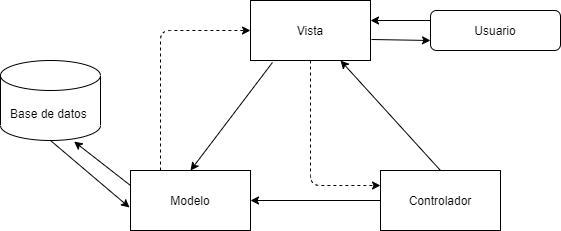
\includegraphics[width=12cm, keepaspectratio]{img/model-vista-controlador.png}
	\caption{Estructura de las relación modelo-vista-controlador.}\label{fig:arquitectura}
\end{figure}

\section{Módulo Vistas-Controlador}
Este módulo es el encargado de recibir y gestionar las peticiones recibidas desde el módulo Templates, gestionarlas, consultar con el módulo Models y preparar las respuestas para el usuario. Django dispone de herramientas muy útiles para la gestión y respuesta de peticiones web, de tal manera que definir las funciones del servidor cada vez que un usuario accede a una URL y generar las respuestas es limpio, sencillo, escalable. 
Las URL y como se gestionan las respuestas se define a continuación: 

\begin{itemize}
	\item \textbf {Home}: Como muchas otras aplicaciones que existen, cuando se introduce la URL con el nombre completo del dominio sin añadir ningún directorio tras este, se redirige esta petición a la página principal o home, donde se simplemente se hace una pequeña introducción al proyecto y te permite iniciar Gymkhana App. 
	\item \textbf {/start}: Cuando inicias la Gymkhana desde el home te lleva automáticamente a esta URL, donde primero este módulo comprueba si existen juegos disponibles en la base de datos, y si es así los muestra. El usuario puede elegir uno de estos juegos y enviar una petición GET con el identificador del juego elegido. 
	\item \textbf {/challenge}: Cuando se accede a este directorio se recoge la petición GET del usuario con el juego elegido, y si vienes de un reto anterior o acaba de empezar el juego. Así podemos elegir cual de los diferentes retos que componen un juego mostrar, siempre comprobando que todos los datos existan en la base de datos para evitar posibles errores. Una vez elegido el reto a mostrar se le muestra a el reto donde el usuario debe introducir la respuesta al mismo para avanzar. 
	\item \textbf {/response}: Una vez el usuario ha rellenado la repuesta al reto se envía una petición tipo GET con la información contenida del reto al que pertenece, el juego, sí ha habido una reto del mismo juego anterior y la respuesta al reto. En caso de ser correcta el servidor redirigirá al usuario bien al nuevo reto, si se está jugando a un juego con varios retos, o una pantalla en la que indica que ha finalizado correctamente el juego y desde ahí el usuario podrá regresar al menú principal para poder elegir otros juegos, o repetir el mismo. Por otro lado, si la respuesta no es correcta, enviará al usuario a una pantalla donde se indica que la respuesta es incorrecta y te dejará volver a intentar el reto o salir al menú de juegos.
\end{itemize}

Django cuenta con muchas funciones y respuestas que vienen ya integradas, como por ejemplo poder responder a peticiones que provocan errores genéricos como tipo HTTP 404 (Not Found) entre otros, de esta manera todas las peticiones que se hacen al servidor en caso de encontrar la información requerida en la base de datos la aplicación captura este error y devuelve un ERROR 404 genérico de Django, que aparte hace terminar el resto de procesos en curso, haciendo a la aplicación mucho más robusta ante errores. 


\section{Módulo Templates-Vistas}
El módulo de Templates es el que forma la interfaz de usuario de la aplicación. Cada vista de la aplicación, o página que el usuario acaba visualizando está compuesta por un template o plantilla HTML sobre la que se aplica un estilo con CSS. Trabajar con plantillas en Django hace que la aplicación sea escalable y el código quede ordenado. En muchos casos la plantilla es reutilizable si se parametrizan adecuadamente, a su vez, la capa de estilo esta muy bien aislada gracias a Boostrap, de manera que se puede separar muy bien la parte programática del desarrollo de la parte encargada del diseño y el estilo evitando así tener que aplicar estilo a cada una de las páginas implicadas en el desarrollo. 

La aplicación de Gymkhana App se apoya principalmente sobre cinco principales views: home, start, challenge, succes y wrong.
\subparagraph{Home}
Es la página principal que el usuario ve cuando accede a la web. Tiene una cabecera y un pie de página que comparten todas las paginas de la aplicación. En la cabecera hay dos enlaces ocultos que redirigirán al usuario bien a la página principal de la aplicación Gymkhana App, o a la web oficial de la organización UML. En el pie de página se muestra información relativa a la ETSIT como localización y enlaces ocultos para poder visitar la cuenta de Twitter, y la web oficial de la ETSIT. También aparece la licencia de uso de la plantilla de Boostrap elegida. En cuanto al contenido de esta página se limita a una presentación sencilla y limpia del proyecto, con un botón bien visible al usuario que será el que le permita avanzar y adentrarse en Gymkhana App. 
\subparagraph{Start}
Esta página actúa de forma de menú y muestra los juegos que hay disponibles en la aplicación, los lista ordenadamente de manera descendientes, y cada juego tiene un botón con el que el usuario puede interactuar, pulsando el mismo accede a dicho juego.  
\subparagraph{Challenge} 
En esta página muestra un único reto, que se compone de un nombre o título, una pregunta y una imagen con un diagrama UML que debe estar relacionado con el reto. Esta vista tiene también un campo que el usuario debe rellenar con la respuesta planteada al reto y un botón par enviar la petición que más tarde procesará el módulo Vistas-Controlador.
\subparagraph{Success}
Una vez enviada la respuesta a un reto, si eta es correcta te redirigirá a esta página donde puedes ver un texto dando la enhorabuena al usuario. Dependiendo del juego te mostrará un botón para volver al menú de juegos o al siguiente reto si el juego estaba compuesto por varios. 
\subparagraph{Wrong}
En contraposición a la anterior plantilla, esta mostrará al usuario un comentario haciéndole saber que la respuesta no es correcta, pero también animándolo a que lo vuelva a intentar. Esta plantilla solo mostrará dos botones, uno para volver a intentar el reto que ha fallado y otro para volver al menú de juegos en caso de que el usuario desista y de por perdido el reto. 

NOTA: PODEMOS AÑADIR PANALLAZOS CON TODA LA INTERFAZ EN LOS ANEXOS PARA RELLERNAR

\subsection{Internacionalización}
Django también ofrece de manera relativamente sencilla la posibilidad de añadir internacionalización a las plantillas. Este proceso consiste en traducir todo el texto que aparece en las plantillas. 

En este proyecto, el idioma original que se eligió para desarrollar las plantillas fue el inglés, pero con el proceso de internacionalización también está disponible en castellano. La idea básica de la internacionalización o I18N es marcar aquellas cadenas de texto que deben ser traducidas. Estas cadenas se guardan en un diccionario, donde se añade la traducción al idioma o idiomas deseados, de esta manera cuando un usuario seleccione un idioma, mostrará estas cadenas de texto marcadas en el lenguaje que le corresponda al usuario. 

En el diccionario aparte de todas las cadenas de texto que se muestran en las diferentes plantillas, también están guardadas las respuestas a los retos. Esta es la única manera de poder procesar las respuesta de los usuarios en diferentes idiomas y comprobar que coinciden con la respuesta de un reto concreto. 

De la misma manera, para poder traducir las imágenes de los diagramas UML que se muestran, cada diagrama tiene que estar disponible en dos idiomas diferentes, es decir cada diagrama está representado por dos imágenes, una en inglés y otra en castellano, así se seleccionará la imagen correspondiente dependiendo del idioma del usuario. 

\section{Módulo Models-Modelo}
Este módulo es el que gestiona la información de la aplicación Gymkhana App, toda la información de la aplicación está contenida en una base de datos. El gestor de base de datos utilizado es, en este caso, SQLite versión 3. Este sistema de base de datos es un sistema de base de datos relacional y es por defecto el que utiliza Django, no obstante se permite cambiar a otros modelos fácilmente. Se ha decidido utilizar este gestor precisamente por la sencillez y compatibilidad con Django, con SQLite la base de datos completa se encuentra en un solo archivo totalmente autocontenido, sin dependencias externas ademas admite concurrencia decir que permite que múltiples procesos tengan el archivo de base de datos abierto y leer a la vez. En  en la figura~\ref{fig:diagarma_ER} se puede ver el diagrama entidad-relación que define la base de datos de la aplicación, el proyecto de Django tiene más tablas a parte de las que se muestran, pero el resto son propias de la arquitectura de Django así que no nos centraremos en ellas. Las tablas que componen la base de datos de la aplicación se describen a continuación:


\begin{itemize}
	\item \textbf {Users}: En esta tabla se almacenan los usuarios registrados en Gymkhana App. Dispone de los siguientes campos: 
	\begin{itemize}
		\item \textbf {name}: Indica el nombre del usuario. 
		\item \textbf {email}: La dirección de correo electrónico con la que se registra el usuario. 
		\item \textbf {admin}: Un campo que indica si este usuario tiene privilegios de administrador o no. 
	\end{itemize}

	\item \textbf {Diagrams}: Esta tabla contiene los tipos de diagramas que pueden aparecer en los retos, estos tipos de diagramas se limitan a los mencionados en el apartado 3.1 de este documento.  
	\begin{itemize}
		\item \textbf {type}: Indica el nombre general del tipo de diagrama UML. 
		\item \textbf {description}: La descripción del tipo de diagrama asociado que se puede extender hasta diez mil caracteres. 
	\end{itemize}
	
	\item \textbf {Challenges}: Tabla que almacena los retos de los que se componen los juegos que maneja la aplicación. 
	\begin{itemize}
		\item \textbf {name}: Nombre que se le da a cada reto.
		\item \textbf {question}: Pregunta clave sobre el reto específico. 
		\item \textbf {awnser}: Respuesta a la pregunta clave. 
		\item \textbf {diagram}: Diagrama UML, en formato imagen a la que está asociado el reto. 
		\item \textbf {creator}: Usuario que ha creado este reto. 
		\item \textbf {diagram type}: El tipo de diagrama UML al que esta asociado el diagrama de este reto. 
	\end{itemize}
	
	\item \textbf {Games}: Tabla que almacena los distintos juegos, estos juegos son principalmente una colección de uno o varios retos. 
	\begin{itemize}
		\item \textbf {title}: Nombre o título del juego. 
		\item \textbf {challenges}: Uno o varios retos de los contenidos en la tabla Challenges. 
		\item \textbf {creator}: Usuario que ha creado el juego. 
	\end{itemize}
	
\end{itemize}

\begin{figure}
	\centering
	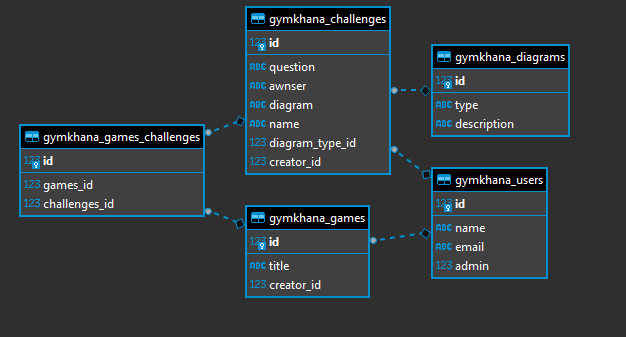
\includegraphics[width=16cm, keepaspectratio]{img/ghymkhana_ER.png}
	\caption{Diagrama entidad-relación de la aplicación Ghymkhana App.}\label{fig:diagarma_ER}
\end{figure}



%%%%%%%%%%%%%%%%%%%%%%%%%%%%%%%%%%%%%%%%%%%%%%%%%%%%%%%%%%%%%%%%%%%%%%%%%%%%%%%%
%%%%%%%%%%%%%%%%%%%%%%%%%%%%%%%%%%%%%%%%%%%%%%%%%%%%%%%%%%%%%%%%%%%%%%%%%%%%%%%%
% EXPERIMENTOS Y VALIDACIÓN %
%%%%%%%%%%%%%%%%%%%%%%%%%%%%%%%%%%%%%%%%%%%%%%%%%%%%%%%%%%%%%%%%%%%%%%%%%%%%%%%%

\cleardoublepage

\chapter{Experimentos y validación}

Este capítulo se introdujo como requisito en 2019. 
Describe los experimentos y casos de test que tuviste que implementar para validar tus resultados. 
Incluye también los resultados de validación que permiten afirmar que tus resultados son correctos. 


%%%%%%%%%%%%%%%%%%%%%%%%%%%%%%%%%%%%%%%%%%%%%%%%%%%%%%%%%%%%%%%%%%%%%%%%%%%%%%%%
%%%%%%%%%%%%%%%%%%%%%%%%%%%%%%%%%%%%%%%%%%%%%%%%%%%%%%%%%%%%%%%%%%%%%%%%%%%%%%%%
% RESULTADOS %
%%%%%%%%%%%%%%%%%%%%%%%%%%%%%%%%%%%%%%%%%%%%%%%%%%%%%%%%%%%%%%%%%%%%%%%%%%%%%%%%

\cleardoublepage
\chapter{Resultados}

En este capítulo se incluyen los resultados de tu trabajo fin de grado.

Si es una herramienta de análisis lo que has realizado, aquí puedes poner ejemplos de haberla utilizado para que se vea su utilidad.


%%%%%%%%%%%%%%%%%%%%%%%%%%%%%%%%%%%%%%%%%%%%%%%%%%%%%%%%%%%%%%%%%%%%%%%%%%%%%%%%
%%%%%%%%%%%%%%%%%%%%%%%%%%%%%%%%%%%%%%%%%%%%%%%%%%%%%%%%%%%%%%%%%%%%%%%%%%%%%%%%
% CONCLUSIONES %
%%%%%%%%%%%%%%%%%%%%%%%%%%%%%%%%%%%%%%%%%%%%%%%%%%%%%%%%%%%%%%%%%%%%%%%%%%%%%%%%

\cleardoublepage
\chapter{Conclusiones}
\label{chap:conclusiones}


\section{Consecución de objetivos}
\label{sec:consecucion-objetivos}

Esta sección es la sección espejo de las dos primeras del capítulo de objetivos, donde se planteaba el objetivo general y se elaboraban los específicos.

Es aquí donde hay que debatir qué se ha conseguido y qué no. 
Cuando algo no se ha conseguido, se ha de justificar, en términos de qué problemas se han encontrado y qué medidas se han tomado para mitigar esos problemas.

Y si has llegado hasta aquí, siempre es bueno pasarle el corrector ortográfico, que las erratas quedan fatal en la memoria final.
Para eso, en Linux tenemos aspell, que se ejecuta de la siguiente manera desde la línea de \emph{shell}:

\begin{verbatim}
  aspell --lang=es_ES -c memoria.tex
\end{verbatim}

\section{Aplicación de lo aprendido}
\label{sec:aplicacion}

Aquí viene lo que has aprendido durante el Grado/Máster y que has aplicado en el TFG/TFM. Una buena idea es poner las asignaturas más relacionadas y comentar en un párrafo los conocimientos y habilidades puestos en práctica.

\begin{enumerate}
  \item a
  \item b
\end{enumerate}


\section{Lecciones aprendidas}
\label{sec:lecciones_aprendidas}

Aquí viene lo que has aprendido en el Trabajo Fin de Grado/Máster.

\begin{enumerate}
  \item Aquí viene uno.
  \item Aquí viene otro.
\end{enumerate}


\section{Trabajos futuros}
\label{sec:trabajos_futuros}

Ningún proyecto ni software se termina, así que aquí vienen ideas y funcionalidades que estaría bien tener implementadas en el futuro.

Es un apartado que sirve para dar ideas de cara a futuros TFGs/TFMs.


%%%%%%%%%%%%%%%%%%%%%%%%%%%%%%%%%%%%%%%%%%%%%%%%%%%%%%%%%%%%%%%%%%%%%%%%%%%%%%%%
%%%%%%%%%%%%%%%%%%%%%%%%%%%%%%%%%%%%%%%%%%%%%%%%%%%%%%%%%%%%%%%%%%%%%%%%%%%%%%%%
% APÉNDICE(S) %
%%%%%%%%%%%%%%%%%%%%%%%%%%%%%%%%%%%%%%%%%%%%%%%%%%%%%%%%%%%%%%%%%%%%%%%%%%%%%%%%

\cleardoublepage
\appendix
\chapter{Manual de usuario}
\label{app:manual}

Esto es un apéndice.
Si has creado una aplicación, siempre viene bien tener un manual de usuario.
Pues ponlo aquí.

\chapter{Anexo I: Ejemplos de Diagramas UML}
% Contenido del anexo I
Aqui vienen las fotitos de los diagramas UML 

{\footnotesize
	\begin{verbatim}
		@inproceedings{robles2005self,
			title={Self-organized development in libre software:
				a model based on the stigmergy concept},
			author={Robles, Gregorio and Merelo, Juan Juli\'an 
				and Gonz\'alez-Barahona, Jes\'us M.},
			booktitle={ProSim'05},
			year={2005}
		}
	\end{verbatim}
}


\cleardoublepage


%%%%%%%%%%%%%%%%%%%%%%%%%%%%%%%%%%%%%%%%%%%%%%%%%%%%%%%%%%%%%%%%%%%%%%%%%%%%%%%%
%%%%%%%%%%%%%%%%%%%%%%%%%%%%%%%%%%%%%%%%%%%%%%%%%%%%%%%%%%%%%%%%%%%%%%%%%%%%%%%%
% BIBLIOGRAFIA %
%%%%%%%%%%%%%%%%%%%%%%%%%%%%%%%%%%%%%%%%%%%%%%%%%%%%%%%%%%%%%%%%%%%%%%%%%%%%%%%%

\cleardoublepage

% Las siguientes dos instrucciones es todo lo que necesitas
% para incluir las citas en la memoria
\bibliographystyle{abbrv}
\bibliography{memoria}  % memoria.bib es el nombre del fichero que contiene
% las referencias bibliográficas. Abre ese fichero y mira el formato que tiene,
% que se conoce como BibTeX. Hay muchos sitios que exportan referencias en
% formato BibTeX. Prueba a buscar en http://scholar.google.com por referencias
% y verás que lo puedes hacer de manera sencilla.
% Más información: 
% http://texblog.org/2014/04/22/using-google-scholar-to-download-bibtex-citations/

%https://es.wikipedia.org/wiki/Lenguaje_unificado_de_modelado
%versiones uml https://www.omg.org/spec/UML/
%https://www.omg.org/spec/UML/2.5.1/PDF
%https://docs.djangoproject.com/en/3.2/

\end{document}
